\chapter{Statistics: Sampling}\label{Statistics: Sampling}

\begin{figure}[h]
    \centering
    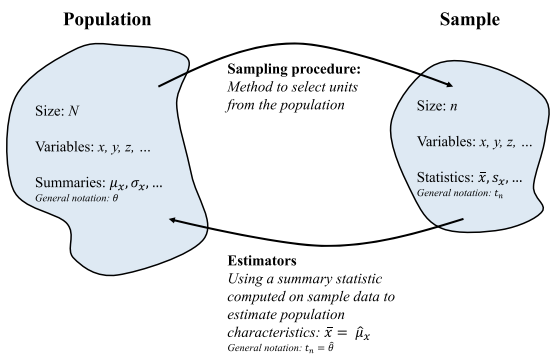
\includegraphics[width=\linewidth, height=4cm, keepaspectratio]{Pictures/statistics/population-and-sample.png}
\end{figure}

\begin{customTableWrapper}{1.5}
\begin{table}[h]
    \centering
    \begin{tabular}{|l|c|c|}
        \hline
        \customTableHeaderColor
        & \textbf{Population} & \textbf{Sample}\\
        \hline

        \textbf{Size} & $N$ & $n$ \\
        \hline

        \textbf{Variables} & $x,y,z,\cdots$ & $x,y,z,\cdots$ \\
        \hline

        \textbf{Summaries/ Statistics} & $\mu_x,\sigma_x,\cdots$ & $\bar{x}, s_x, \cdots$\\
        \hline

        \textbf{General Notation} & $\theta$ & $t_n$\\
        \hline
    \end{tabular}
\end{table}
\end{customTableWrapper}


\section{Convenience Sampling \cite{ism-1}} \label{Convenience Sampling}

\begin{enumerate}
    \item collects only units from the population that can be \textbf{easily obtained}

    \item may provide a \textbf{biased} sample

    \item often justified by using the argument of \textbf{population homogeneity}
\end{enumerate}

\section{Haphazard Sampling \cite{ism-1}}
\label{Haphazard Sampling}

\begin{enumerate}
    \item Despite the feeling of randomness when performing haphazard sampling, often the resulting sample is not truly random.

\end{enumerate}


\section{Purposive Sampling \cite{ism-1}}\label{Purposive Sampling}

\begin{enumerate}
    \item tries to sample units for a specific purpose. 

    \item This means that the collection of units is focused on one or more particular characteristics and hence it implies that only units that are more alike are sampled.
\end{enumerate}


\section{Simple Random Sampling \cite{ism-1}}\label{Simple Random Sampling}

\begin{customTableWrapper}{2.5}
\begin{longtable}{|p{5cm}|p{9cm}|}
    \hline\endfirsthead
    \hline\endhead
    \hline\endfoot
    \hline\endlastfoot

    \textbf{Number of possible samples} & \( \dfrac{N!}{n!(N-n)!} \) \\
    \hline

    \textbf{Probability that $S_k$ is selected} & $\pi_k = \dfrac{1}{K}$ \\
    \hline

    \textbf{Probability that a specific unit is part of the sample} & $\dfrac{n}{N}$ \\
    \hline

    \textbf{Mean ($\mathbb{E}(T)$)} & $
        \mathbb{E}(T) = 
        \dfrac{1}{K} \dsum_{k=1}^{K}
        \bar{x}_k 
        =
        \dfrac{1}{nK} \dsum_{k=1}^{K}
        \dsum_{i \in S_k} x_i
        =
        \dfrac{1}{N} \dsum_{i=1}^{N} x_i
        = \mu
    $ \\[2ex]
    \hline

    \textbf{Estimator of Mean ($\bar{x}_k$)} & $
        \bar{x}_k=
        \dfrac{1}{n} \dsum_{i=1}^{n} x_i
    $ \\[2ex]
    \hline

    \textbf{Bias} & $
        bias(c\bar{x}_k) = (c-1)\mu
        \quad\quad\quad
        bias(\bar{x}_k) = 0
    $ \\[1ex]
    \hline

    \textbf{MSE ($MSE(c\bar{x}_k)$)} & 
    \tableenumerate{
        \item 
        $
            MSE(c\bar{x}_k) 
            = [(c-1)\mu]^2 +
            c^2 \sigma^2 \dParenBrac{\dfrac{N}{N-1} }\dParenBrac{( 1-\dfrac{n}{N} }\dfrac{1}{n}
        $

        \item 
        $MSE(\bar{x}_k) 
            = \sigma^2 \dParenBrac{\dfrac{N}{N-1} }\dParenBrac{( 1-\dfrac{n}{N} }\dfrac{1}{n}
        $ 
    } \\
    \hline

    \textbf{Estimator of MSE ($\hat{MSE}(\bar{x}_k)$)} & $
        \hat{MSE}(\bar{x}_k) = \dParenBrac{\dfrac{N-n}{Nn} }s_k^2
    $\\[1ex]
    \hline

    \textbf{Variance ($\sigma^2$)} & $
        \sigma^2 = \dfrac{1}{N} \dsum_{i=1}^{N}
        (x_i - \mu)^2
    $\\[1ex]
    \hline

    \textbf{Estimator of Variance ($s_k^2$)} & $
        s_k^2 = \dParenBrac{\dfrac{1}{n-1}} \dsum_{i\in S_k}
        (x_i - \bar{x}_k)^2
    $\\[1ex]
    \hline

    \textbf{SE ($SE(c\bar{x}_k)$)} & $
        SE(c\bar{x}_k) = \sqrt{
            c^2 \sigma^2 
            \dParenBrac{ \dfrac{N}{N-1} }
            \dParenBrac{ 1-\dfrac{n}{N} }
            \dfrac{1}{n}
        }
    $\\[1ex]
    \hline
\end{longtable}
\end{customTableWrapper}

\section{Systematic Sampling \cite{ism-1}}\label{Systematic Sampling}

\begin{enumerate}
    \item Population should be divided into $n$ groups and the order of the units (if some order exists) should be maintained (or otherwise fix the order).

    \item each group consists of $m$ units (thus the population size is $N = nm$) \textbf{ordered} from $1$ to $m$ in each group.
    \[
        m \in \dCurlyBrac{1,2,\cdots,N}
    \]

    \item from each of the $n$ groups the $k$th unit is collected, forming the sample of $n$ units. 
    \[
        S_k = \dCurlyBrac{ k, k+m,k+2m,\cdots,k+(n-1)m }
        \hfill
        (k \in \dCurlyBrac{1,2,\cdots,m})
    \]
\end{enumerate}

\begin{customTableWrapper}{2}
\begin{longtable}{|p{5cm}|p{9cm}|}
    \hline\endfirsthead
    \hline\endhead
    \hline\endfoot
    \hline\endlastfoot

    \textbf{Probability of selecting $S_k$} & $\dfrac{1}{m}$\\[1ex]
    \hline

    \textbf{Mean ($\mu$)} & $
        \mu = \dfrac{1}{N}
        \dsum_{h=1}^{m}
        \dsum_{i=1}^{n} 
        x_{h+m(i-1)}
    $\\[1ex]
    \hline

    \textbf{Estimator of Mean ($\bar{x}_k$)} & $
        \bar{x}_k = 
        \dfrac{1}{n} \dsum_{i=1}^{n}
        x_{h+m(i-1)}
    $\\[1ex]
    \hline

    \textbf{Variance ($\sigma^2$)} & $
        \sigma^2 = 
        \dfrac{1}{N}
        \dsum_{k=1}^{m}
        \dsum_{i=1}^{n}
        (x_{k+m(i-1)} - \mu)^2
    $\\[1ex]
    \hline

    \textbf{Estimator of Variance ($s_k^2$)} & $
        s_k^2 = \dParenBrac{\dfrac{1}{n-1}}
        \dsum_{i=1}^{n}
        (x_{k+m(i-1)} - \bar{x}_k)^2
    $\\[1ex]
    \hline

    \textbf{Bias} & $bias(\bar{x}_k) = 0$\\
    \hline

    \textbf{MSE} & $
        MSE = \sigma^2 -
        \dfrac{1}{N}
        \dsum_{h=1}^{m}
        \dsum_{i=1}^{n}
        (x_{h+m(i-1)} - \bar{x}_h)^2
    $\\[1ex]
    \hline
\end{longtable}
\end{customTableWrapper}

\section{Stratified Sampling \cite{ism-1}}\label{Stratified Sampling}

\begin{enumerate}
    \item numbers of units across the \textbf{subpopulations} $S_h$ (called \textbf{strata}\indexlabel{strata}) are (substantially) different $N_h$

    \item selecting the same fraction/ proportion of the units from each stratum we are certain that each stratum is included in the sample, and represents the population

    \item If the ratio of the sample size $n_h$ and stratum size $N_h$ is the same across all strata, each unit in the population has the same probability of being collected in the sample. This type of stratified sampling is called \textbf{proportional stratified sampling}\indexlabel{proportional stratified sampling}.

    \item[] $S_h = \dCurlyBrac{ S_{h,1}, S_{h,2},\cdots, S_{h,N_h} }$

    \item[] $K_h = \dfrac{N_h!}{n_h!(N_h-n_h)!}$

    \item[] $w_h = \dfrac{N_h}{N}$

    \item[] $
        K_S = 
        \dfrac{N_1!}{n_1!(N_1-n_1)!} 
        \times
        \dfrac{N_1!}{n_1!(N_1-n_1)!} 
        \times
        \cdots
        \times
        \dfrac{N_M!}{n_M!(N_M-n_M)!}
        =
        \dprod_{M}^{i=1} \dfrac{N_i!}{ni!(N_i-n_i)!}
    $

    \item[] $
        \dsum_{i=1}^{M} N_i = N
        \quad\quad
        \dsum_{i=1}^{M} n_i = n
    $


\end{enumerate}

\begin{customTableWrapper}{1}
\begin{longtable}{|p{5cm}|p{9cm}|}
    \hline\endfirsthead
    \hline\endhead
    \hline\endfoot
    \hline\endlastfoot

    number of possible samples that can be collected with stratified random sampling & $K_S$\\
    \hline

    \textbf{Mean ($\mu_h$)} & $
        \mu_h = \dfrac{1}{N_h} 
        \dsum_{i=1}^{N_h} x_{hi}
    $\\[1ex]
    \hline

    \textbf{Estimator of Mean ($\bar{x}_{h,k}$)} & 
    \tableenumerate{
        \item $
            \bar{x}_{h,k} = \dfrac{1}{n_h} 
            \dsum_{i\in S_{h,k}} x_{hi}
        $

        \item $
            \bar{x}_{k} = \dsum_{h=1}^{M}
            w_h\bar{x}_{h,k}
            = \dsum_{h=1}^{M}
            \dParenBrac{\dfrac{N_h}{N}}
            \left(
                \dfrac{1}{n_h} 
                \dsum_{i=1}^{n_h} x_{hi}
            \right)
        $ \vspace{0.2cm}
    } \\
    \hline

    \textbf{Variance ($\sigma_h^2$)} & 
    \tableenumerate{
        \item $
            \sigma_h^2=\dfrac{1}{N_h}
            \dsum_{i=1}^{N_h}
            (x_{hi} - \mu_{h})^2
        $

        \item $
                \sigma^2 
                = \dfrac{1}{N}
                \dsum_{h=1}^{M}
                \dsum_{i=1}^{N_h}
                (x_{hi}-\mu)^2
                =\dsum_{h=1}^{M} w_h\sigma_h^2 +
                \dsum_{h=1}^{M} w_h(\mu_h - \mu)^2
        $  \vspace{0.1cm}
        
        \item[] (within) \& (between) variances
    } \\
    \hline

    \textbf{Estimator of Variance ($s_{h,k}^2$)} & $
        s_{h,k}^2 = 
        \dfrac{1}{n_h - 1}
        \dsum_{i\in S_{h,k}}
        (x_{hi} - \bar{x}_{h,k})^2
    $\\
    \hline

    \textbf{Bias} & 0\\
    \hline

    \textbf{MSE} & 
    \tableenumerate{
        \item $
            MSE = \dsum_{h=1}^{M}
            \left[
                \left(
                    \dfrac{N_h^2(N_h-n_h)}{n_h(N_h-1)N^2}
                \right)
                \sigma_h^2
            \right]
        $ \vspace{0.2cm}
        
        \item $
            MSE(\bar{x}_k) = \dsum_{h=1}^{M}
            w_h^2 MSE(\bar{x}_{h,k})
            = \dsum_{h=1}^{M}
            \dfrac{N_h(1-f_h)w_h^2\sigma_h^2}{(N_h-1)n_h}
        $ \vspace{0.2cm}
    }
    \\
    \hline

    \textbf{Estimator of MSE ($\hat{MSE}$)} & $
        \hat{MSE}(\bar{x}_k) = \dfrac{1}{n_h}
        \dsum_{h=1}^{M}
        (1-f_h)w_h^2 s_{h,k}^2
    $\\[1ex]
    \hline

    \textbf{SE} & $
        SE(cT) = c\cdot SE(T)
    $\\[1ex]
    \hline
    
    \textbf{Esimator of SE ($\hat{SE}$)} & $
        \hat{SE}(\bar{x}_{h,k}) =
        \sqrt{\dfrac{1-f_h}{n_h}}s_{h,k}
    $\\[1ex]
    \hline
\end{longtable}
\end{customTableWrapper}


\section{Cluster Sampling \cite{ism-1}}\label{Cluster Sampling}

\begin{enumerate}
    \item Directly sampling units from populations is not feasible.

    \item random sampling of groups or clusters of units in the population

    \item Cluster sampling can be less representative than sampling units directly.

    \item cluster sampling introduces a specific structure in the sample which should also be addressed when the data is being analyzed.

    \item The cluster structure introduces two sources of variation in the data being collected.
    \begin{enumerate}
        \item Within-cluster variation
        \item Between-cluster variation
    \end{enumerate}

    \item Cluster sampling is in a way related to stratified sampling
\end{enumerate}

\subsection{Single-stage Cluster Sampling \cite{ism-1}} \label{Single-stage Cluster Sampling}

\begin{enumerate}
    \item uses a random sample of the clusters and then all units from these clusters are selected (aka \textbf{primary cluster units}\indexlabel{primary cluster units})

    \item $x_{hi}$ the value on variable $x$ for unit $i$ in cluster $h$
    \[
        N = \dsum_{h=1}^{M} N_h
    \]

    
\end{enumerate}

\begin{longtable}{|p{5cm}|p{9cm}|}
    \hline\endfirsthead
    \hline\endhead
    \hline\endfoot
    \hline\endlastfoot

    \textbf{Mean ($\mu$)} & $
        \mu = \dfrac{1}{N}
        \dsum_{h=1}^{M}
        \dsum_{i=1}^{N_h}
        x_{hi}
    $\\[1ex]
    \hline

    \textbf{Estimator of Mean} & \begin{minipage}{8cm}
        \vspace{0.1cm}
        $
            \bar{x}_h = \mu_h
            \quad\quad
            \bar{x} = \dfrac{1}{m}
            \dsum_{h=1}^{m} \bar{x}_h
        $\\
        \begin{enumerate}
            \item cluster sizes are all not equal
            \[
                \displaystyle
                \sum_{h=1}^{m}
                \left(
                    \frac{N_h}{
                        \sum_{h=1}^{m} N_h
                    }
                \right)\bar{x}_h
            \]
            \[
                \dfrac{1}{M}\dsum_{h=1}^{M}\mu_h
                =
                \dsum_{h=1}^{M}
                \dsum_{i=1}^{N_h}
                \dfrac{x_{hi}}{MN_h}
            \]

            \item cluster sizes are all equal
            \[
                \dfrac{M}{mN}
                \dsum_{h=1}^{m} N_h\bar{x}_h
            \]

            \item Cluster sizes are fixed
            \[
                \bar{x}_F =
                \left( 
                    \dsum_{h=1}^{m} N_h\bar{x}_h
                \right) / \left( 
                    \dsum_{h=1}^{m} N_h
                \right)
            \]

            \item Cluster sizes are random:
            \[
                \bar{x}_R= \dParenBrac{ \dfrac{M}{mN} }
                \dsum_{h=1}^{m} N_h\bar{x}_h
            \]
        \end{enumerate}
        \vspace{0.01cm}
    \end{minipage}
    \\[1ex]
    \hline

    \textbf{Bias} & \begin{minipage}{8cm}
        \begin{enumerate}
            \item cluster sizes are all not equal: $\geq 0$
            \item cluster sizes are all equal: $0$
        \end{enumerate}
        \vspace{0.1cm}
    \end{minipage}\\
    \hline

    \textbf{MSE} & \begin{minipage}{8cm}
        \vspace{0.2cm}
        \begin{enumerate}
            \item cluster sizes are all not equal:
            \[
                \sim\dfrac{M^2}{m(M-1)N^2}
                \dParenBrac{1- \dfrac{m}{M} }
                \dsum_{h=1}^{M}
                N_h^2(\mu_h - \mu)^2
            \]

            \item cluster sizes are all equal:
            \[
                \dfrac{M^2}{m(M-1)N^2}
                \dParenBrac{1- \dfrac{m}{M} }
                \dsum_{h=1}^{M}
                (N_h\mu_h - N\mu/M)^2
            \]
        \end{enumerate}
        \vspace{0.01cm}
    \end{minipage}\\
    \hline

    \textbf{Estimator of MSE} & \begin{minipage}{8cm}
        \vspace{0.2cm}
        \begin{enumerate}
            \item Cluster sizes are random
            \[
                \hat{MSE}(\bar{x}_R) =
                \dfrac{M-m}{N^2Mm(m-1)}
                \dsum_{h=1}^{m}
                (MN_h\bar{x}_h - N\bar{x}_R)^2
            \]
        \end{enumerate}
        \vspace{0.1cm}
    \end{minipage}\\
    \hline

    \textbf{Estimator of SE} & \begin{minipage}{8cm}
        \vspace{0.2cm}
        \begin{enumerate}
            \item Cluster sizes are random
            \[
                \hat{SE}(\bar{x}_R) =
                \sqrt{\hat{MSE}(\bar{x}_R)}
            \]
        \end{enumerate}
        \vspace{0.1cm}
    \end{minipage}\\
    \hline
\end{longtable}

\textbf{Note}:
\begin{enumerate}
    \item $\bar{x},\bar{x}_F $ and $\bar{x}_R$ are all \textbf{equal} when the cluster sizes are all \textbf{equal}.

    \item When the cluster means are truly heterogeneous, the random approach provides the smallest standard error.

\end{enumerate}


\subsection{Multiple stages Cluster Sampling \cite{ism-1}} \label{Multiple stages Cluster Sampling}

\begin{enumerate}
    \item the units from the sampled clusters are also randomly sampled instead of taking all units from the cluster.

    \item Number of stages can increase in general to any level, depending on the application.

\end{enumerate}



\begin{longtable}{|p{2cm}|p{12cm}|}
    \hline\endfirsthead
    \hline\endhead
    \hline\endfoot
    \hline\endlastfoot

    \textbf{Estimator} & \begin{minipage}{11cm}
        \vspace{0.2cm}
        \begin{enumerate}
            \item $2$-stage clustering with all $N_h$ are equal:
            \[
                \dfrac{M}{mN} \dsum_{h=1}^{m}
                N_h\bar{x}_h
            \]

            \item $2$-stage clustering with all $N_h$ are \textbf{NOT} equal:
            \[
                \dsum_{h=1}^{m}
                \left( 
                    \frac{N_h}{\sum_{h=1}^{m} N_h} 
                \right)\bar{x}_h
            \]
            
        \end{enumerate}
        \vspace{0.2cm}
    \end{minipage}\\
    \hline

    \textbf{Bias} & \begin{minipage}{11cm}
        \vspace{0.2cm}
        \begin{enumerate}
            \item $2$-stage clustering with all $N_h$ are equal: $0$

            \item $2$-stage clustering with all $N_h$ are \textbf{NOT} equal: $\geq 0$
        \end{enumerate}
        \vspace{0.2cm}
    \end{minipage}\\
    \hline

    \textbf{MSE} & \begin{minipage}{11cm}
        \vspace{0.2cm}
        \begin{enumerate}
            \item $2$-stage clustering with all $N_h$ are equal:
            \[
                \dfrac{M}{mN^2} \left[
                    \dParenBrac{1- \dfrac{m}{M} }
                    \dParenBrac{\dfrac{1}{M-1} }
                    \dsum_{h=1}^{M}
                    (N_h\mu_h - N_\mu/M)^2
                    +
                    \dsum_{h=1}^{M}
                    \left(
                        \dfrac{N_h^2 (N_h-n_h)}{n_h(N_h -1)}
                        \sigma_h^2
                    \right)
                \right]
            \]

            \item $2$-stage clustering with all $N_h$ are \textbf{NOT} equal:
            \[
                \sim
                \dfrac{M}{mN^2} \left[
                    \dParenBrac{1- \dfrac{m}{M} }
                    \dParenBrac{\dfrac{1}{M-1} }
                    \dsum_{h=1}^{M}
                    N_h^2(\mu_h - \mu)^2
                    +
                    \dsum_{h=1}^{M}
                    \left(
                        \dfrac{N_h^2 (N_h-n_h)}{n_h(N_h -1)}
                        \sigma_h^2
                    \right)
                \right]
            \]
        \end{enumerate}
        \vspace{0.2cm}
    \end{minipage}\\
    \hline

    
\end{longtable}


\section{Cross-Sectional (population-based) Study \cite{ism-1}}\label{Cross-Sectional (population-based) Study}

\begin{enumerate}
    \item \textbf{simple random sample} (SEE: \fullref{Simple Random Sampling}) of size $n$ is taken from the population

    \item For each unit in the sample both the exposure and outcome are being observed and the units are then summarized into the four cells $(E, D), (E, D^c), (E^c, D)$, and $(E^c, D^c)$.

    \item This way of sampling implies that $Pr(D), Pr(D^c), Pr(E)$ and $Pr(E^c)$ would be unknown before sampling and they are being determined by the probability of outcome and exposure in the population.

    \item if we define the binary variable $x_i$ by $1$ if unit $i$ has both events $E$ and $D$ (thus $E \cap D$) and it is zero otherwise, the estimate of the population proportion $Pr(E \cap D)$ would be the sample average of this binary variable. 

    \item sample average is equal to the number of units in cell $(E, D)$ divided by the total sample size $n$.

\end{enumerate}


\section{Cohort (exposure-based) Study \cite{ism-1}} \label{Cohort (exposure-based) Study}

\begin{enumerate}
    \item Simple random sample is taken from the population of units who are exposed and another simple random sample is taken from the population of units who are unexposed. Thus this way of sampling relates directly to \textbf{stratified sampling} (SEE: \fullref{Stratified Sampling}) with the strata being the group of exposed ($E$) and the group of unexposed ($E^c$).
    
    \item The sample and the population may have very different probabilities.

    \item Despite the fact that we cannot use the joint probabilities in the contingency table as estimates for the population probabilities, the risk difference, the relative risk, and the odds ratio in the sample are all appropriate estimates for the population when a cohort study is used. The reason is that these measures use the conditional probabilities only, where conditioning is done on the exposure. The $Pr(D|E)$ and $Pr(D|E^c)$ in the sample do represent the conditional population probabilities.
\end{enumerate}


\section{Case-control (disease-based) Study \cite{ism-1}} \label{Case-control (disease-based) Study}

\begin{enumerate}
    \item Simple random sample is taken from the population of units having the outcome and from the population of units without the outcome. Thus this way of sampling relates also directly to \textbf{stratified sampling} (SEE: \fullref{Stratified Sampling}) with the strata being the group with outcome ($D$) and the group without outcome ($D^c$). 

    \item Thus for disease-based sampling the probabilities $Pr(D)$ and $Pr(D^c)$ are known before sampling and are fixed in the sample.

    \item The observed probabilities in the sample are inappropriate as estimates for the same probabilities in the population. Thus we cannot estimate how many units in the population have the outcome

    \item we cannot estimate the joint probabilities $Pr(D \cap E), Pr(D \cap Ec), Pr(D \cap E)$, and $Pr(D \cap E)$ in the population from the sample

    \item the conditional probabilities $Pr(D|E)$ and $Pr(D|E^c)$ cannot be determined either
\end{enumerate}


\section{Sample Statistic ($T_n$) \cite{ism-1}}\label{Sample Statistic}

\begin{enumerate}
    \item sample $X_1, X_2, \cdots, X_n$ of size $n$ from a population as a set of \textbf{random variables} all coming from the same distribution function $F$

    \item we will consider the sample $X_1, X_2, \cdots, X_n$ as a set of random variables and $x_1, x_2,\cdots, x_n$ as the set of realizations that we would see or observe if we have conducted the (sampling) experiment

    \item A sample statistic $T_n \in R$ is defined as any function 
    \[
        T_n \equiv T(X_1, X_2,\cdots, X_n)
    \]
    that is applied to the sample $X_1, X_2,\cdots, X_n$
    \begin{enumerate}
        \item As $T_n$ is a function of random variables, it is itself a random variable
        
        \item $t_n = T(x1, x2,\cdots, xn)$
    \end{enumerate}

\end{enumerate}


\begin{longtable}{|p{2cm}|p{12cm}|}
    \hline\endfirsthead
    \hline\endhead
    \hline\endfoot
    \hline\endlastfoot

    \textbf{$p$th moment} & \begin{minipage}{11cm}
        % \vspace{0.1cm}
        \[
            \mathbb{E}(T_n^p) = \int_{\mathbb{R}}
            t^p f_{T_n}(t)dt
        \]
        If $X_i \sim F$:
        \[
            \mathbb{E}(T_n^p) 
            = \dint_{\mathbb{R}}
            t^pf_{T_n}(t)dt =
            \mathbb{E}(T_n^p(X_1,X_2,\cdots,X_n))
        \]
        \[
            = \dint_{\mathbb{R}^n}
            T_n^p(x_1,x_2,\cdots,x_n)f(x_1)f(x_2)\cdots f(x_n) dx_1 dx_2 \cdots dx_n
        \]

        if $p=1$: $\mu(f_{T_n}) = \mathbb{E}(T_n)$
        \vspace{0.2cm}
    \end{minipage}\\
    \hline

    \textbf{$p$th central moment} & $
        \mathbb{E}(T_n - \mu(f_{T_n}))^p
    $\\
    \hline

    \textbf{standard deviation (or standard error)} & 
    \begin{minipage}{11cm}
        \[
            SE = \dfrac{\sigma(f)}{\sqrt{n}}
            \quad\quad\quad
            n \to \infty \Rightarrow
            SE \to 0
        \]
        sample average converges to the population mean $\mu(f)$
        standardized sample average:
        \[
            Z_n 
            = \dfrac{\hat{X} - \mu(f)}{\mu(f)/\sqrt{n}}
            = \dfrac{\sqrt{n}(\hat{X} - \mu(f))}{\mu(f)}
        \]
        mean would be equal to zero: $\mathbb{E}(Z_n) = 0$\\
        variance would be equal to one: $\mathbb{E}(Z_n^2) = 1$
        \vspace{0.2cm}
    \end{minipage}\\
    \hline
\end{longtable}


\subsection{Central Limit Theorem (CLT) \cite{ism-1}} \label{Sample Statistic: Central Limit Theorem (CLT)}

\begin{enumerate}
    \item distribution functions converges to the \textbf{standard normal distribution function}
    \[
        \Phi(z) = \dint_{-\infty}^{z}
        \phi(x)dx
        \quad\quad\quad
        Z_n = \dfrac{\sqrt{n}(\hat{X} - \mu(f))}{\mu(f)}
        \sim \mathcal{N}(0,1)
    \]

    \item Let $X_1, X_2,\cdots, X_n$ be i.i.d. with distribution function $F$ and with mean $\mu(f) = E(X_k)$ and with finite variance $\sigma ^2(f) = E(X_k - \mu(f))^2 < \infty$. 

    \item The distribution function of $\sqrt{n}(\hat{X}-\mu(f))$ converges to the normal distribution function with mean zero and variance $\sigma ^2(f)$
    
    \item the distribution function of $\dfrac{\sqrt{n}(\hat{X} - \mu(f))}{\mu(f)}$ converges to the standard normal distribution function

    \item the distribution function of any statistic of the form $S_n = \dsum_{i=1}^{n} \psi(X_i)/n$ would also converge to a normal distribution function when the mean $\mu _\psi (f) = E(\psi (X_k))$ and variance $\sigma ^2_\psi (f) = E(\psi (X_k) - \mu _\psi (f))^2$ are finite

    \item Using the central limit theorem, $\psi(X_1), \psi(X_2), \cdots, \psi(X_n)$ are i.i.d. and have a finite variance; thus, the statistic $\sqrt{n}(S_n - \mu_\psi(f))$ converges to a \textbf{normal distribution} with mean zero and variance $\sigma^2_\psi(f)$
\end{enumerate}


\subsection{Central Limit Theorem Applied to Variances \cite{ism-1}} \label{sample statistic: Central Limit Theorem Applied to Variances}

\begin{enumerate}
    \item can be applied to the sample variance $S^2$, when the fourth central moment $E(X_k - \mu(f))^4$ exists

    \item Sample variance (re-written):
    \[
        S^2=
        \dfrac{1}{n-1}
        \dsum_{i=1}^{n} (X_i-\mu(f))^2 -
        \dfrac{n}{n-1} (\bar{X} - \mu(f))^2
    \]

    \item applying CLT on $\dfrac{1}{n}
        \dsum_{i=1}^{n} (X_i-\mu(f))^2$:
    \begin{enumerate}
        \item $\psi (x) = (x - \mu (f))2$
    
        \item mean of $\psi (X_i) = (X_i - \mu (f))^2$ is given by 
        \[
            \mu _\psi (f) = E(X_i -\mu (f))^2 = \sigma^2(f)
        \]
        
        \item sample variance:
        \[
        \begin{aligned}
            \sigma ^2_\psi ( f ) 
            &= \mathbb{E}((X_i - \mu( f ))^2 - \sigma ^2( f ))^2
            &= \mathbb{E}(X_i - \mu( f ))^4 - \sigma ^4( f ) 
            &= [\gamma_2( f ) + 2]\sigma ^4( f )
        \end{aligned}
        \]
    
        \item variance of $
            \dfrac{1}{n}
            \dsum_{i=1}^{n} (X_i -\mu( f ))^2
            =
            [\gamma_2( f ) + 2]\sigma^4( f )/n
        $

        \item $
            \dfrac{1}{\sqrt{n}}
            \dsum_{i=1}^{n}
            [(X_i - \mu( f )) ^2 - \sigma^2 ( f )]
            \quad
            \overset{n\to \infty}{\longrightarrow}
            \quad
            \mathcal{N}(0,[\gamma_2( f ) + 2]\sigma^4( f ))
        $

        \item $
            \dfrac{1}{n}
            \dsum_{i=1}^{n} (X_i - \mu(f))^2
        $ 
        is approximately \textbf{normally distributed} with
        \[
            \mathcal{N}(\sigma^2( f ),[\gamma_2( f ) + 2]\sigma^4( f )/N )
        \]
        \[
            \Rightarrow
            \dfrac{1}{n}
            \dsum_{i=1}^{n} (X_i - \mu(f))^2
            \approx
            \mathcal{N}(\sigma^2( f ),[\gamma_2( f ) + 2]\sigma^4( f )/N )
        \]

        \item $\sqrt{n}(\bar{X} - \mu( f ))$ converges to the normal distribution $\mathcal{N}(0, \sigma^2( f ))$
        \[
            \Rightarrow
            (\bar{X} - \mu( f ))^2 
            = [\sqrt{n}(\bar{X} - \mu( f ))]2/n 
            \quad
            \overset{n\to \infty}{\longrightarrow}
            \quad
            0
        \]

        \item $\sqrt{n}(S^2 - \sigma^2( f ))$ converges to a normal distribution $\mathcal{N}(0,[\gamma_2( f ) + 2]\sigma^4( f ))$
    \end{enumerate}

    
\end{enumerate}

\subsection{Asymptotic Confidence Intervals \cite{ism-1}} \label{sample statistic: Asymptotic Confidence Intervals}

\begin{customTableWrapper}{1.5}
\begin{longtable}[H]{l l}
    $F_{T_n}$ & sample distribution function \\

    $x_p( f_{T_n} )$, $x_{1-p}( f_{T_n} )$ & quantiles ($p < 0.5$)\\

    $(x_p( f_{T_n} ), x_{1-p}( f_{T_n} )]$ & interval with probability $1 - 2p$\\

    $\theta$ & population characteristic ($\mu( f )$, $\sigma ( f )$, or $x_p( f )$)\\

    $\tau_n$ & standard error of the sample statistic $T_n$ \\

    $(T_n - \theta )/\tau_n$ & \\

    $z_p = x_p (\phi)$ & quantile of the standard normal distribution\\

    $(\theta + z_p\theta_n, \theta + z_{1-p}\theta_n] = (\theta - z_{1-p}\theta_n, \theta + z_{1-p}\theta_n]$ & interval\\

    $b_2$ & sample excess kurtosis\\
\end{longtable}
\end{customTableWrapper}

\[
\begin{aligned}
    Pr(T_n \in (x_p( f_{T_n} ), x_{1-p}( f_{T_n} )]) 
    &= Pr(T_n \leq x_{1-p}( f_{T_n} )) - Pr(T_n \leq x_p( f_{T_n} ))\\
    &= F_{T_n} (x_{1-p}( f_{T_n} )) - F_{T_n} (x_p( f_{T_n} ))\\
    &= 1 - p - p = 1 - 2p
\end{aligned}
\]

\[
\begin{aligned}
    Pr(T_n \in (\theta  - z_{1-p}\tau_n, \theta  + z_{1-p}\tau n]) 
    &= Pr((T_n - \theta  )/\tau n \in (-z_{1-p},z_{1-p}])\\
    &\approx \Phi (z_{1-p}) - \Phi (-z_{1-p})\\
    &= 1 - p - p = 1 - 2p
\end{aligned}
\]

\[
    Pr(T_n \in (\theta  - z_{1-p}\tau n, \theta  + z_{1-p}\tau n]) =
    Pr(\theta  \in (T_n - z_{1-p}\tau n, T_n + z_{1-p}\tau n])
\]

\begin{enumerate}
    \item asymptotic confidence interval for $\theta$ with confidence level $1 - 2p$:
    \[
        (T_n - z_{1-p}\tau_n, T_n + z_{1-p}\tau_n]
        \hfill
        \text{($\tau_n$ : Standard error)}
    \]

    \item asymptotic $1 - 2p$ confidence interval for the variance $\sigma^2$ is given by:
    \[
        (S^2 - z_{1-p}\hat{\tau}_n, S^2 - z_{1-p}\hat{\tau}_n]
        \hfill
        (\text{estimated standard error : } \tau_n = S^2\sqrt{[b_2 + 2]/n})
    \]

    \item asymptotic confidence interval can be written into the form of $(c_n S^2,C_n S^2]$:
    \[
        \hfill
        cn = 1 - z_{1-p}\sqrt{[b_2 + 2]/n} 
        \hfill
        Cn = 1 + z_{1-p}\sqrt{[b_2 + 2]/n} 
        \hfill
    \]
\end{enumerate}


\subsection{Sample average ($T_n = \bar{X} = \frac{1}{n}\sum_{i=1}^{n} X_i $) \cite{ism-1}}

\subsection{Sample variance ($T_n = S^2 = \frac{1}{n-1}\sum_{i=1}^{n} (X_i - \bar{X})^2$) \cite{ism-1}}

\subsection{Sample standard deviation ($T_n = S = \sqrt{\frac{1}{n-1}\sum_{i=1}^{n} (X_i - \bar{X})^2}$) \cite{ism-1}}

\subsection{Sample skewness ($T_n = b_1 = \frac{1}{n} \sum_{i=1}^{n} (X_i - \bar{X})^3/S^3 $) \cite{ism-1}}

\subsection{Sample excess kurtosis ($T_n = b_2 = \frac{1}{n} \sum_{i=1}^{n} (X_i - \bar{X})^4/S^4 -3$) \cite{ism-1}}

\subsection{Sample minimum $T_n = X_{(1)} = \min\dCurlyBrac{X_1,\cdots,X_n}$ \cite{ism-1}}

\subsection{Sample maximum $T_n = X_{(n)} = \max\dCurlyBrac{X_1,\cdots,X_n}$ \cite{ism-1}}

\subsection*{}

\begin{enumerate}
    \item The order statistics $X_{(1)}, X_{(2)},\cdots, X_{(n)}$ can be used to determine the quantiles $x_p$ of the population:\\
    if $np \in N$, $q_p = [X_{(np)} + X_{(1+np)}]/2$\\
    else, $q_p = X_{( \left \lceil np \right \rceil)}$
\end{enumerate}


\section{Sampling sentences from a language model \cite{nlp-1}}\label{Sampling sentences from a language model}

\begin{enumerate}
    \item Sampling from a distribution means to choose random points according to their likelihood. 

    \item Thus sampling from a language model—which represents a distribution over sentences—means to generate some sentences, choosing each sentence according to its likelihood as defined by the model. 

    \item Thus we are more likely to generate sentences that the model thinks have a high probability and less likely to generate sentences that the model thinks have a low probability.

    \item We choose a random value between $0$ and $1$, find that point on the probability line, and print the word whose interval includes this chosen value. 

    \item We continue choosing random numbers and generating words until we randomly generate the sentence-final token \verb|</s>|.
\end{enumerate}






















